\chapter{ROS 2 Middleware Implementation for WebAssembly}

    The design of a custom middleware implementation, \textsf{rms-wasm}, that can be cross-compiled to WebAssembly modules is divided into three distinct packages as observed in Figure~\ref{fig:rmwwasm}. For this project, these packages were developed in the order shown, starting with \textsf{rmw-wasm-cpp}.

    \begin{figure}[htbp]
        \centering
        \vspace{1em}
        \begin{tikzpicture}
            \node (pkg) [
                rectangle,
                rounded corners,
                fill = shade05,
                text height = 7cm,
                align = justify,
                minimum width = 14cm,
                text width = 13.5cm,
            ] {\textsf{rmw-wasm}};

            \node (rwc) [
                packBox,
                yshift = 2.5cm,
                fill = shade15,
                ] {\textsf{rmw-wasm-cpp}};

            \node (wcpp) [
                packBox,
                yshift = 0.5cm,
                fill = shade15,
                ] {\textsf{wasm-cpp}};

            \node (wjs) [
                packBox,
                yshift = -2.5cm,
                fill = shade15,
                ] {\textsf{wasm-js}};
            
            \node (ems) [
                rectangle,
                yshift = -1cm,
                xshift = 2cm,
                ] {\texttt{emscripten::val}};

            \draw[thick] (rwc) -- (wcpp);
            \draw[thick] (wcpp) -- (wjs);

        \end{tikzpicture}
        \vspace{1em}
        \caption{Architecture of custom middleware implementation to target WebAssembly.}
        \label{fig:rmwwasm}
    \end{figure}

    \section{rmw-wasm-cpp}

        The first package, \textsf{rmw-wasm-cpp}, works as the ``adapter'' between \ac{ROS} 2 and the designed middleware. This package implements all of the functions required for \textsf{rmw} as described in Section~\ref{ssec:minimal}. The source code for this package is entirely written in C++ and can be found: TODO: 

        TODO: add diagram

        TODO: mention yaml conversion, add diagram?

    \section{wasm-cpp}

        The role of \textsf{wasm-cpp} is to implement the middleware and to function as a bridge to JavaScript modules. This package, along with \textsf{wasm-js} constitute the middleware implementation without the adapter, and thus, they can function independently of \textsf{rmw-wasm-cpp}. 

        The \ac{ROS} elements in this package build on top of each other, where the smallest unit is a \texttt{Participant}. Any \ac{ROS} subscriber, publisher, service server, service client, action server, or action client is simply a \texttt{Participant} with a specific role. Each \texttt{Participant} must have a valid name which follows the \ac{ROS} guidelines (TODO: add ref for valid names). For publishers and subscribers, this name is their respective topic name. And for servers and clients, the name corresponds to the service or action name.  Upon initialization, each \texttt{Participant} also receives a unique ID or \texttt{gid} which is used to keep track of individual participants. A class diagram illustrating the relations between the different elements is shown in Figure~\ref{fig:classes}.

        \begin{figure}[htbp]
            \centering
            \vspace{1em}
            \begin{tikzpicture}%[show background grid]
                \begin{abstractclass}[text width=5cm]{Participant}{0,0}
                    \attribute{- name : String}
                    \attribute{- role : String}
                    \attribute{- gid  : String}
    
                    \operation{- is\_valid\_name( )}
                    \operation{- is\_valid\_role( )}
                    \operation{- registration( )}
                    \operation{- deregistration( )}
                \end{abstractclass}
    
                \begin{class}[text width=5cm]{Publisher}{-5,-6}
                    \inherit{Participant}
                    \attribute{- name = topic\_name}
                    \attribute{- role = publisher}
                    \operation{+ publish(message : String)}
                \end{class}
    
                \begin{class}[text width=5cm]{Subscriber}{5,-6}
                    \inherit{Participant}
                    \attribute{- name = topic\_name}
                    \attribute{- role = subscriber}
                    \operation{+ get\_message( ) : String}
                \end{class}
    
                \begin{class}[text width=6.5cm]{ServiceServer}{-4,-11}
                    \inherit{Participant}
                    \attribute{- name = service\_name}
                    \attribute{- role = service\_server}
                    \operation{+ take\_request( ) : String}
                    \operation{+ send\_response(response : String)}
                \end{class}
    
                \composition{ServiceServer}{}{}{Publisher}
                \composition{ServiceServer}{}{}{Subscriber}
    
                \begin{class}[text width=6.5cm]{ServiceClient}{4,-11}
                    \inherit{Participant}
                    \attribute{- name = service\_name}
                    \attribute{- role = service\_client}
                    \operation{+ send\_request(request : String)}
                    \operation{+ take\_response( ) : String}
                    \operation{+ is\_service\_available( ) : Bool}
                \end{class}
    
                \composition{ServiceClient}{}{}{Publisher}
                \composition{ServiceClient}{}{}{Subscriber}
    
            \end{tikzpicture}
            \vspace{1em}
            \caption{A class diagram}
            \label{fig:classes}
        \end{figure}
        

        Subscribers and publishers are the simplest type of participants. And each of them only has one function; a publisher needs to be able to \textit{publish} a message, and a subscriber must be able to \textit{retrieve} the message from a specific topic. The messages which the publisher handles are yaml strings. These messages are then passed to \textsf{wasm-js} by using \texttt{emscripten::val} which transliterates JavaScript code into C++ (TODO: add ref). Figure~\ref{fig:publish} shows how these functions are implemented to create a \textit{bridge} between the two packages.

        \begin{figure}[htbp]
            \centering
            \begin{lstlisting}[language=C++]
// wasm_cpp/src/publisher.cpp
#include <emscripten/emscripten.h>
#include <emscripten/val.h>
...
emscripten::val js_publish = emscripten::val::module_property("publishMessage");
bool is_published = js_publish(yaml_message, topic_name).as<bool>();
\end{lstlisting}

            % To match syntax hightlight
            \begin{lstlisting}[language=C++] 
// wasm_js/src/pre.js
Module["publishMessage"] = function publishMessage(message, topic_name)
{
    if (message.startsWith("data:")) {
    self.postMessage({
        command: "publish",
        topic:    topic_name,
        message: message
    });
    }

    return true;
}
\end{lstlisting}
            \caption{Publisher sending a message to JavaScript for publishing.}
            \label{fig:publish}
        \end{figure}

    Conversely, the subscriber \textit{waits} for a response from \textsf{wasm-js} which will indicate that a new message has been published to the topic in question. The response message type is coerced into a yaml string to send back to \textsf{rmw-wasm-cpp}. This process is illustrated in Figure~\ref{fig:retrieve}.

    \begin{figure}[htbp]
        \centering
        \begin{lstlisting}[language=C++]
// wasm_cpp/src/subscriber.cpp
emscripten::val js_retrieve = emscripten::val::module_property("retrieveMessage");
emscripten::val js_response = js_retrieve(topic_name).await();
std::string yaml_message = js_response.as<std::string>();
\end{lstlisting}    
        \caption{Subscriber retrieving a message from JavaScript.}
        \label{fig:retrieve}
    \end{figure}

    With the configuration described, subscribers and publishers do not necessarily need to be aware of the existence of other participants within the same topic name. That is to say, a publisher can send messages even when there are no subscribers, and a subscriber can listen to a topic even when there are no messages published. Additionally, this allows multiple publishers to publish to the same topic simultaneously with different \ac{ROS} message types since all messages are handled as strings.

    Services are constructed from publishers and subscribers. A service server and a server client each have one publisher and one subscriber. Before a service client can call a service, it must verify that the service server is available to process a request. This is accomplished by making a query to \textsf{wasm-js} which keeps track of all available entities. If the service server is available, then the service client can \textit{publish} a request to the service request topic. Meanwhile, the service server is \textit{subscribed} to the service request topic to receive the request. Once the service server processes the request, the response tis \textit{published} to the service response topic. And lastly, the service client \textit{subscribed} to the response topic will retrieve the response. This process is summarized in Figure~\ref{fig:service}.

    \begin{figure}[htbp]
        \centering
        \vspace{1em}
        \begin{tikzpicture}
            \node (clt) [
                box,
                minimum width=3.5cm,
                text depth=3cm,
                xshift=-4cm,
                fill=shade20,
            ] {Service Client};

            \node (cltpub) [
                box,
                minimum width=3cm,
                minimum height=1cm,
                xshift=-4cm,
                yshift=0.5cm,
                fill=shade05,
            ] {Publisher};

            \node (cltsub) [
                box,
                minimum width=3cm,
                minimum height=1cm,
                xshift=-4cm,
                yshift=-1cm,
                fill=shade05,
            ] {Subscriber};

            \node (srv) [
                box,
                minimum width=3.5cm,
                text depth=3cm,
                xshift=4cm,
                fill=shade20,
            ] {Service Server};

            \node (srvsub) [
                box,
                minimum width=3cm,
                minimum height=1cm,
                xshift=4cm,
                yshift=0.5cm,
                fill=shade05,
            ] {Subscriber};

            \node (srvpub) [
                box,
                minimum width=3cm,
                minimum height=1cm,
                xshift=4cm,
                yshift=-1cm,
                fill=shade05,
            ] {Publisher};

            \node (t1) [
                box,
                minimum width=3cm,
                minimum height=1cm,
                yshift=0.5cm,
            ] {Request Topic};

            \node (t2) [
                box,
                minimum width=3cm,
                minimum height=1cm,
                yshift=-1cm,
            ] {Response Topic};

            \draw [arrow] (cltpub) -- (t1);
            \draw [arrow] (t1) -- (srvsub);
            \draw [arrow] (srvpub) -- (t2);
            \draw [arrow] (t2) -- (cltsub);

        \end{tikzpicture}
        \vspace{1em}
        \caption{Data flow between \ac{ROS} service client and server.}
        \label{fig:service}
    \end{figure}

    Analogously to services, action servers and clients are handled in the same manner with the addition that action servers will continuously publish feedback to the action response topic until the request being processed is completed.



%%%%%%%%%%%%%%%%%%%%%%%%%%%%%%%%%%%%%%%%%%%%%%%%%%%%%%%%%%%%%%%%%%%%%%%%%%%%%%%%

    \section{wasm-js}

        The last piece of the puzzle is \textsf{wasm-js}. This package is written in JavaScript and its role is to launch and track all the participating entities, and to store and distribute all \ac{ROS} messages accordingly.


    \subsection{Web Workers}

        Given that processes on a browser run on a single ``main thread'', \textsf{wasm-js} uses \textit{web workers} to launch the requested \ac{ROS} nodes. Web workers run in background threads and thus, they do not interfere with the user interface while performing tasks~\cite{workers}. 

        \begin{figure}[htbp]
            \centering
            \begin{tikzpicture}
                \node (thread) [
                    rectangle,
                    rounded corners,
                    draw = textColor,
                    text depth = 4cm,
                    minimum width = 4cm,
                    fill = igmrLightBlue!30!bgColor,
                ] {Main Thread};

                \node (w1) [
                    webBox,
                    xshift = -5cm,
                    yshift = 1cm,
                ] {ROS Node 1 \\ \footnotesize{web worker}};

                \node (w2) [
                    webBox,
                    xshift = -5cm,
                    yshift = -2cm,
                ] {ROS Node 2 \\ \footnotesize{web worker}};

                \node (w3) [
                    webBox,
                    xshift = 5cm,
                    yshift = 1cm,
                ] {ROS Node 3 \\ \footnotesize{web worker}};

                \node (w4) [
                    webBox,
                    xshift = 5cm,
                    yshift = -2cm,
                ] {ROS Node 4 \\ \footnotesize{web worker}};

            \end{tikzpicture}
            \caption{TODO: Web Worker communications}
            \label{fig:webworker}
        \end{figure}

        

    \subsection{Message Stacks}

        \begin{figure}[htbp]
            \centering
            \begin{subfigure}[t]{0.32\textwidth}
                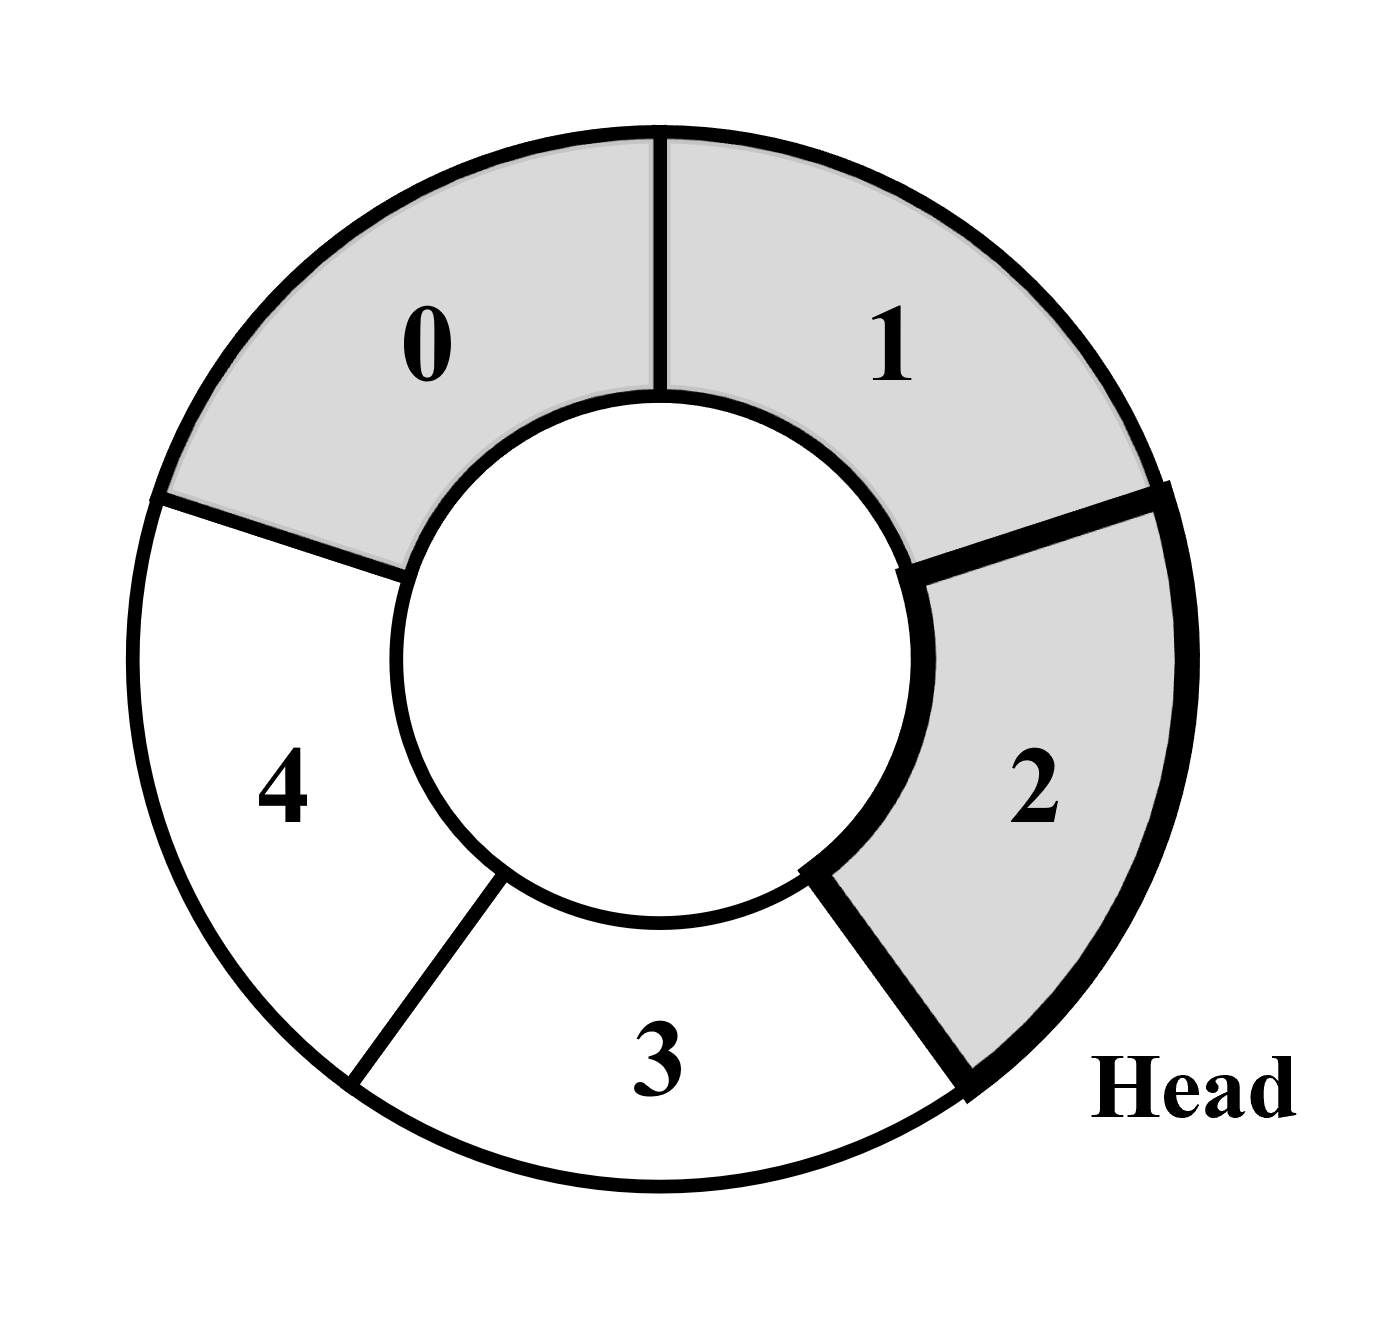
\includegraphics[height=0.9\textwidth]{07_stack0.png}
                \caption{Filling stack}
            \end{subfigure}
            \begin{subfigure}[t]{0.32\textwidth}
                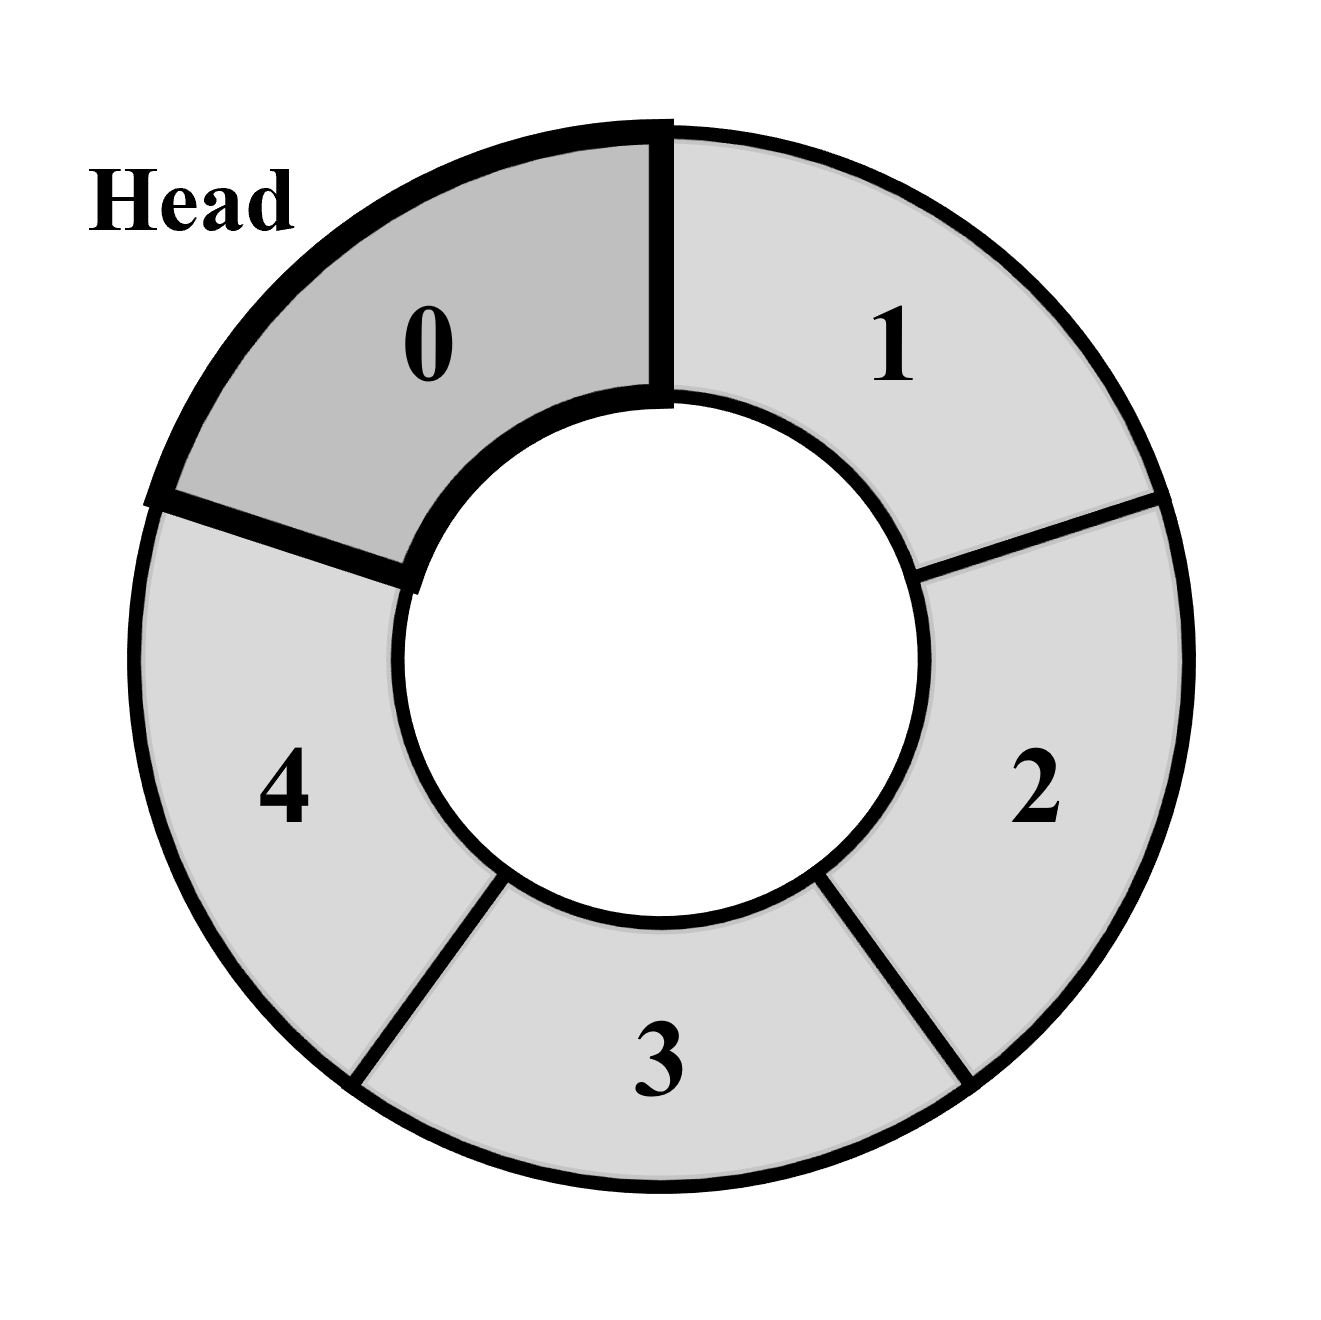
\includegraphics[height=0.9\textwidth]{07_stack1.png}
                \caption{Overwriting stack}
            \end{subfigure}
            \begin{subfigure}[t]{0.32\textwidth}
                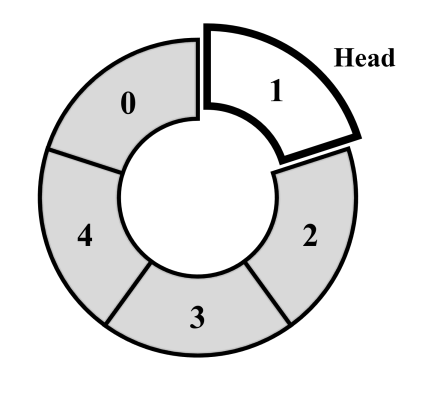
\includegraphics[height=0.9\textwidth]{07_stack2.png}
                \caption{Reading stack}
            \end{subfigure}
            \caption{Modified Circular Stack, \ac{LIFO}}
            \label{fig:circleStack}
        \end{figure}

    - Web workers, what are they? why are they needed?
    - Communication channels
    - Registry of topics/subs/pubs
    - Message handling

